\subsection{Testkonzept Software}\label{sec:testkonzeptSoftware}

Für einen einwandfreien Betrieb ist das Testing der Software einer der wichtigsten Bestandteile der Validierung. Dieses Kapitel wird in die Abschnitte \glqq PWM Signal\grqq, \glqq Verhalten der Statemachine\grqq, \glqq Kommunikation zwischen Bluetooth und Beacon\grqq wie auch \glqq Funktionalität der SD-Karte\grqq geteilt.

\subsubsection{PWM Signal}\label{sec: Validierung PWM Signal}

Das PWM Signal wurde mit dem Gleichen Signal wie das LC-Filter validiert. Dabei wurden sowohl die beiden PWM Kanäle mit dem KO aufgezeichnet wie in \ref{fig Signal PWM Ausgänge} zu sehen ist, sowie das gefilterte Signal. 

\begin{figure}[H]
	\begin{center}
		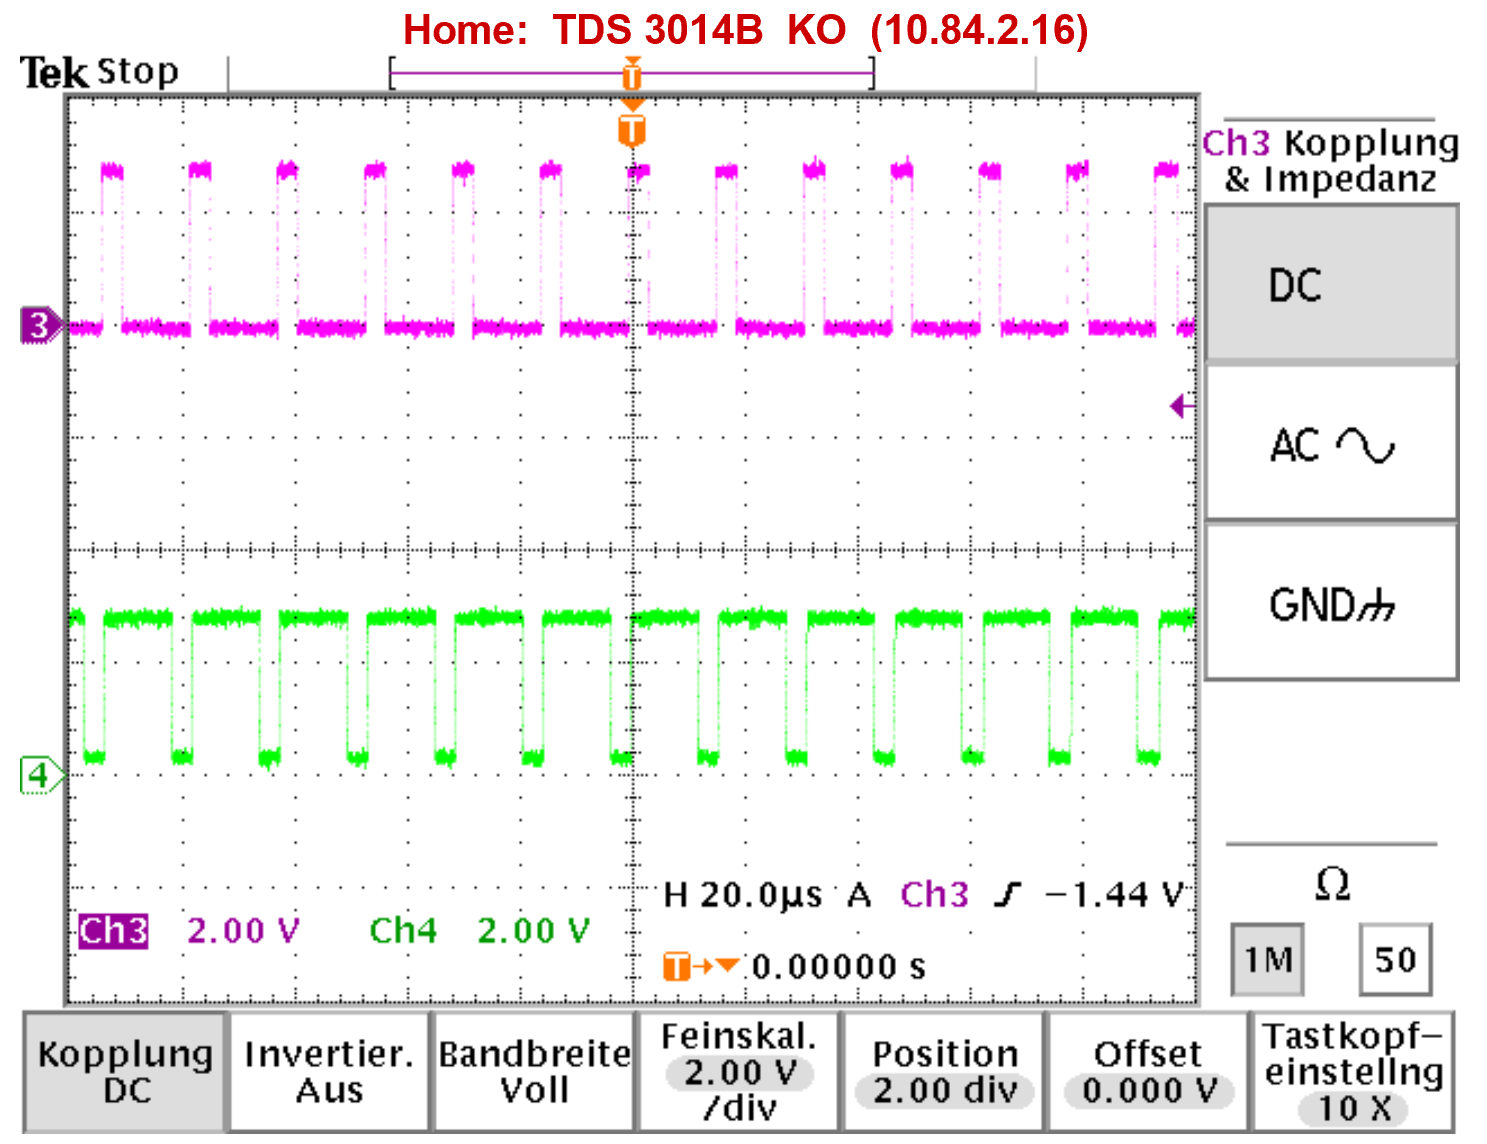
\includegraphics[width=120mm]{data/PWM_Signal_500Hz_Mono_mit_Infos.png}
		\caption[PWM Signal beider PWM Ausgänge]{PWM Signal beider PWM Ausgänge} %picture caption
		\label{fig:Signal PWM Ausgänge}
	\end{center}
\end{figure}


Aus \ref{fig:Signal PWM Ausgänge} ist ersichtlich, dass die beiden PWM Signale zwar invertiert zu einander stehen aber auch zeitlich (knapp knapp $4\mu s$) verschoben sind. Diese Zeitverschiebung hat jedoch keinen hörbaren Effekt und kann somit vernachlässigt werden.\\
Um die Einstellungen des PWM-Moduls aus \ref{sec:audioPWM} zu validieren, wurde ein $500Hz$ Sinus Signal mit dem KO abgebildet. Das entstandene Resultat ist in nachfolgender Abbildung \ref{fig:PWM Topval 500 Stereo} ersichtlich.

\begin{figure}[H]
	\begin{center}
		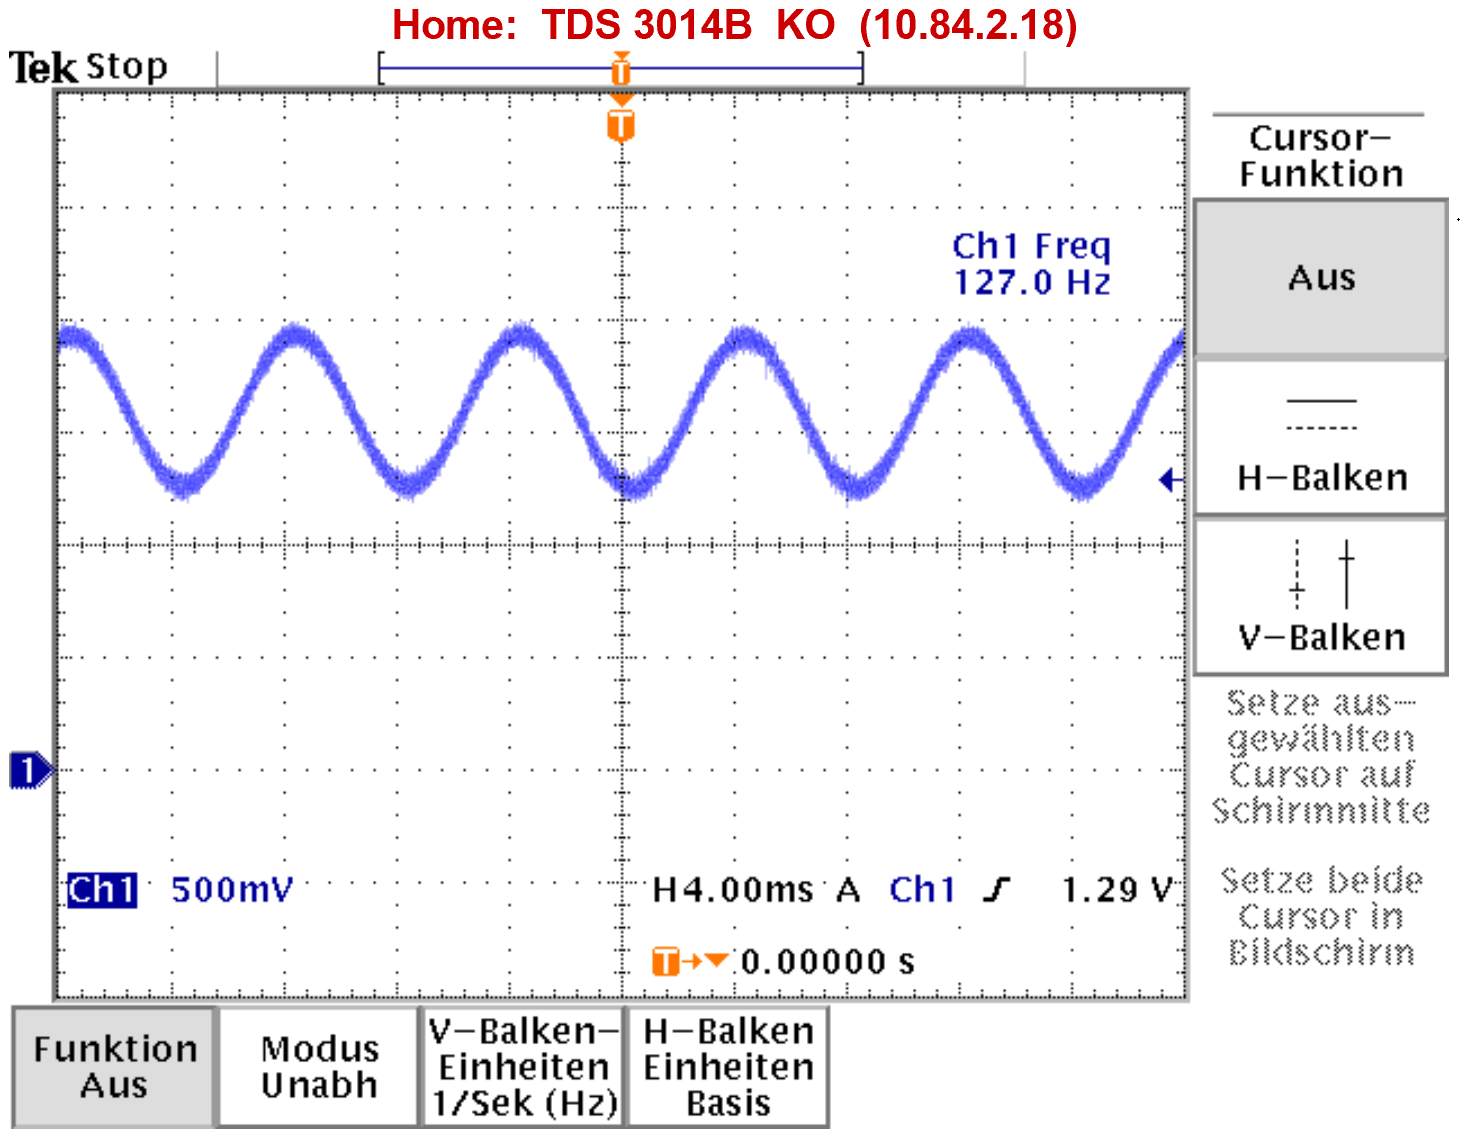
\includegraphics[width=120mm]{data/TOPVAL_Stereo_500.png}
		\caption[PWM auf $32kHz$ eingestellt]{PWM auf $32kHz$ eingestellt} %picture caption
		\label{fig:PWM Topval 500 Stereo}
	\end{center}
\end{figure}


Es ist augenfällig, dass die Frequenz des Signals nun nur $127Hz$ anstatt den angelegten $500Hz$ beträgt, war einem Faktor von rund $4$ entspricht. Um die gewünschten $500Hz$ zu erreichen, wurde der top value aus Kapitel \ref{sec:PWM initialisieren} von $500$ auf $125$ herunter gesetzt. Das entstandene Resultat ist in Abbildung \ref{fig:PWM Topval 125 Stereo} ersichtlich.

\begin{figure}[H]
	\begin{center}
		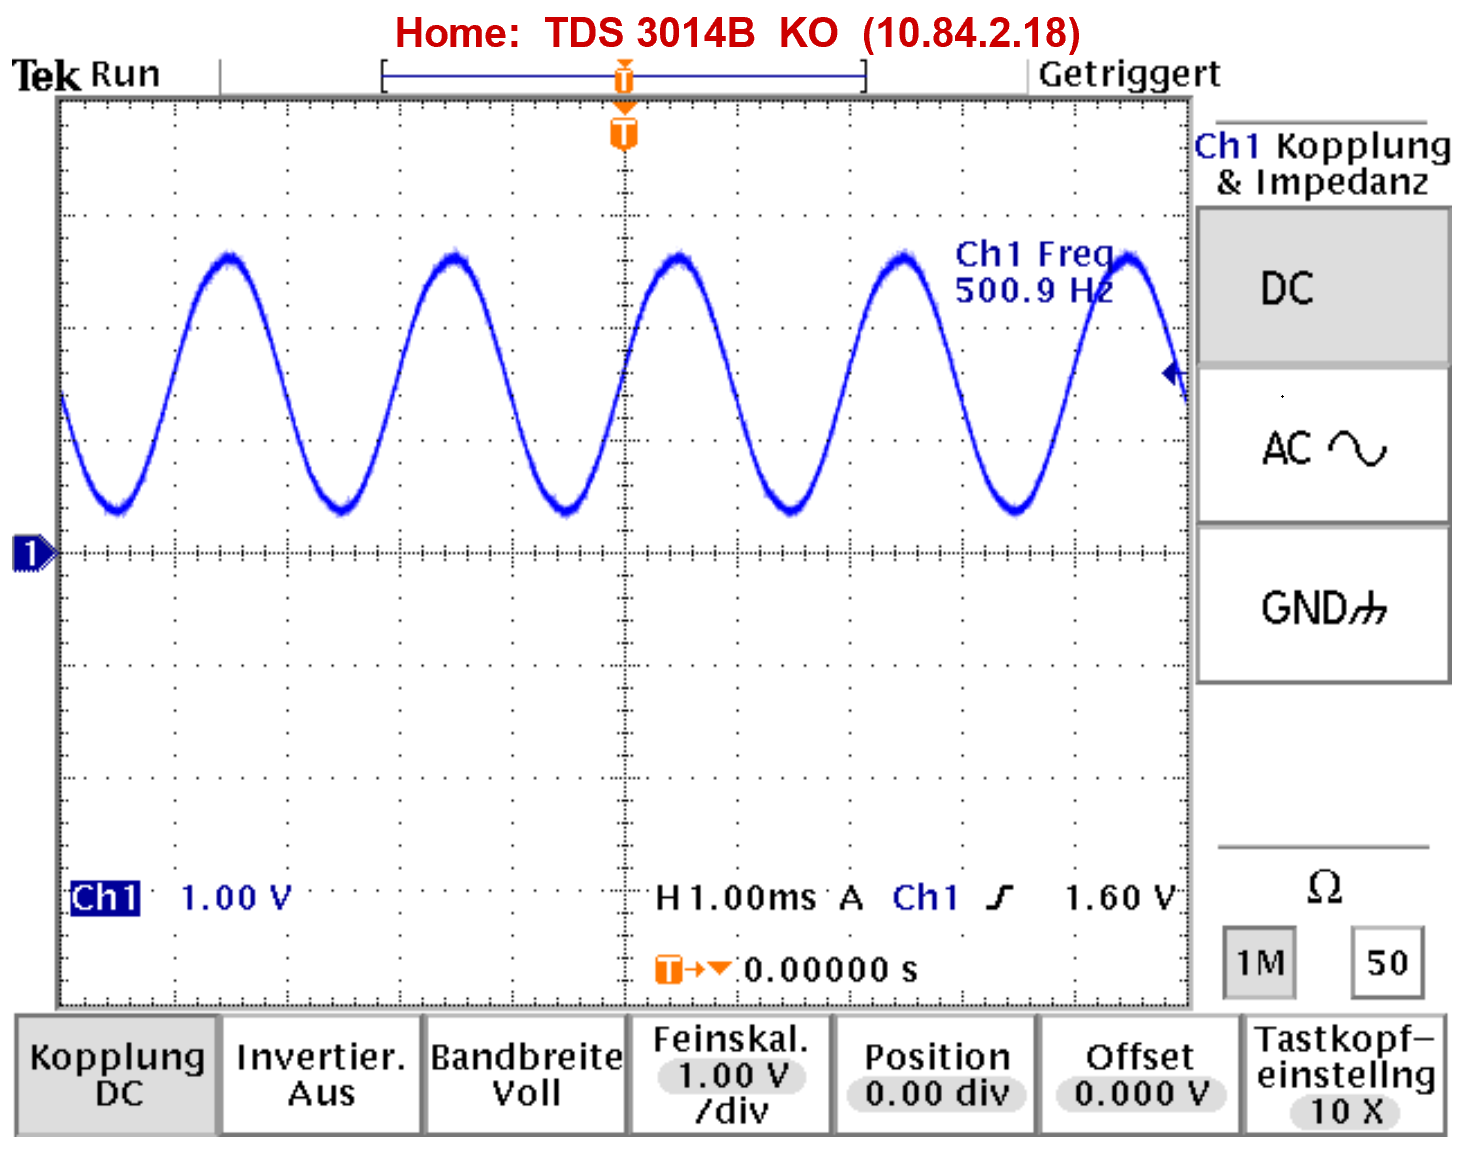
\includegraphics[width=120mm]{data/TOPVAL_Stereo_125.png}
		\caption[PWM auf $128kHz$ eingestellt]{PWM auf $128kHz$ eingestellt} %picture caption
		\label{fig:PWM Topval 125 Stereo}
	\end{center}
\end{figure}

Es ist ersichtlich, dass nun das Sinus Signal mit $500Hz$ schwingt. Da die Berechnungen einen top value von $500$ ergeben, deutet dies auf einen Fehler im Code, in der Audiodatei oder auf einen Überlegungsfehler hin. Es wurde herausgefunden, dass die Tests fälschlicherweise mit einer stereo Audiodatei durchgeführt wurden. Da jedoch nur ein Kanal angesteuert wird, ergibt sich ein Faktor $2$ unterschied zu den Berechnungen. Dieser Test wurde folglich noch einmal mit einer mono Audiodatei durchgeführt, wobei der top value gemäss unseren Erwartungen um den Faktor $2$ vom berechneten Wert abweicht.

\subsubsection{Statemachine}
Die Statemachine wurde auf ihr Verhalten hin getestet. Dabei wurden alle States mithilfe von Flags einmal erzwungen, wobei folgende States nicht korrekt funktionierten:

\begin{itemize}
	\item ADC-Batterie 
	\item Shutdown
	\item Merken Liste Löschen
	\item Charge
\end{itemize}

Es gilt anzumerken, dass diese \glqq fehlerhaften States\grqq in der Statemachiene eigentlich funktionieren, jedoch ihre Aufgabe nicht erfüllen können, da sie aus zeitlichen Gründen nicht implementiert wurden. Die Implementierung dieser States würden bei der Weiterverfolgung dieses Projektes als zusätzlicher Arbeitsschritt implementiert werden.

\subsubsection{Bluetooth}
Das Bluetooth Modul wurde mit verschiedenen Beacons getestet. Dabei is aufgefallen, dass bei der gleichzeitigen Verwendung von mehreren Beacons, welche mit unterschiedlichen Sendeintervallen senden, dies zu grösseren Problemen führt. Es dominieren die Beacons mit schnellerer Sendefrequenz, wobei die langsameren überblendet werden. Aus diesem Grund ist es zu empfehlen, dass die Abstände der Beacons gemäss Abbildung \ref{fig:ref_felder} angewendet werden.

\begin{figure}[H]
	\begin{center}
		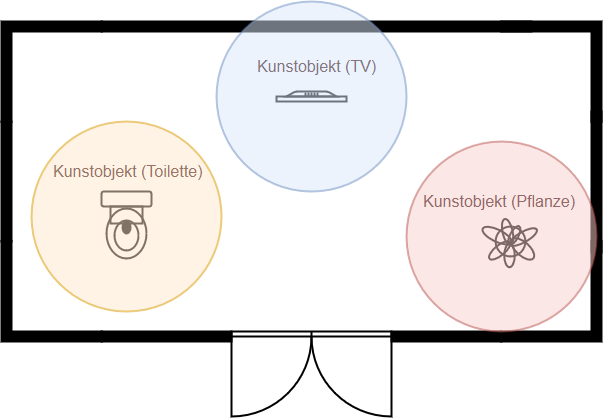
\includegraphics[width=120mm]{data/validierung_software_ref_felder.png}
		\caption[Überlappung der Referenz-Felder]{Überlappung der Referenz-Felder} %picture caption
		\label{fig:ref_felder}
	\end{center}
\end{figure}

\subsubsection{SD-Karte}
Das SD-Karten Modul hat alle Anforderungen erfüllt. Das lesen und schreiben ist problemlos möglich und funktionierte ohne weiteres. Einziger Makel weist die Funktion \glqq Merken\grqq (welche vom \glqq Like Button\grqq aufgerufen wird) auf. Hierbei ist es nicht möglich, ein gemerktes Kunstobjekt wieder zu löschen. Dafür ist es notwendig die SD-Karte aus dem Gerät zu nehmen und sie neu zu konfigurieren. Zudem kann man ein Kunstobjekt gleich mehrmals in die selbe \glqq Merkliste\grqq einfügen, was zwar keine Probleme im Gerät auslöst, aber vom Handlich her nicht sehr schön ist.


